
%==========================================================
\section{Introduction}

\section{Nomenclatures}

\begin{table}[!htb]
  \caption{Nomenclatures System}
  \centering
  \begin{tabular}{||c|c||}
    \hline
    $P$   & Population \\
    \hline
    $\text{GDP}$ & Gross Domestic Product \\
    \hline
    $\text{GAP}$ & Cross Agricultural Product \\
    \hline
    $\text{AWC}$ & Agricultural Water Consumption per year \\
    \hline
    $\text{IWC}$ & Industrial Water Consumption per year \\
    \hline
    $\text{DWC}$ & Domestic Water Consumption per year \\
    \hline
    $\text{TWR}$ & Total Water Resource \\
    \hline
    $\text{SWR}$ & total Surface Water Resource \\
    \hline
    $\text{UWR}$ & total Underground Water Resource \\
    \hline

    $\text{WWD}$ & Waste Water Discharge \\
    \hline

    $A$          & Annual water supplies per person \\
    \hline
  \end{tabular}
\end{table}

\section{Model of water supply ability}
  When it come to the water supply ability of a region, a country or even the world. We often use the measurement called annual water supplies per person($A$) for description\cite{AbilityMeasure}. We can set three levels to classify the ability of several regions:
  \begin{table}[!htb]
    \centering
    \begin{tabular}{|c||c|c|}
    \hline
    level 1   & $A>1700$ & Sufficient \\
    \hline
    level 2   & $1700>A>1000$ & stressful \\
    \hline
    level 3   & $1000>A$ & scarce \\
    \hline
    \end{tabular}
  \end{table}

To cover the internal dynamics of the water flow and the water storage change, we introduce following model.

  \subsection{Model introduction}
    Water circulation is a rather complicated process, which make it almost impossible for us to design a purely fundamental model to include all the variables and their relations. Nevertheless, if we just collect all the data and using fitting method as our predicting model, it will be too trivial and old-fashioned. To solve this paradox, we introduce a phenomenological model which is quite normal in particle physics and other related field. Our model includes two main parts:
    \begin{itemize}
      \item prominent external parameters: a several statistical parameters about a region like population, GDP and so on.
      \item internal dynamic process: a several dynamical relations between external parameters and internal parameters like water consumption ,water recycle and evolution equations of water storage and related variables.
    \end{itemize}


    The dynamics part of our model is inspired by the water cycle(figure \ref{water cycle})\cite{WaterCycle}
    \begin{figure}[!h]
    \begin{center}
    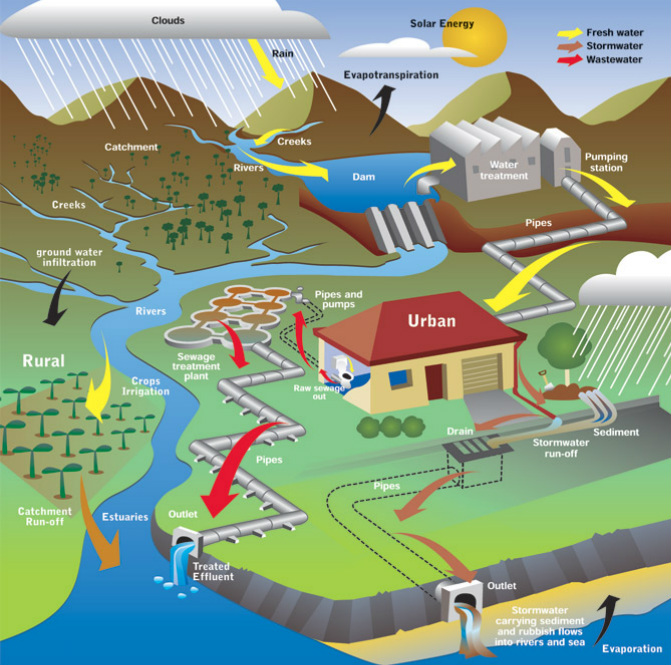
\includegraphics[width = 12cm]{picture/UrbanWaterCycle.jpg}
    \caption{water cycle}
    \label{water cycle}
    \end{center}
    \end{figure}



\section{China's water scarcity}
  According to the UN water scarcity map\cite{WaterScarcityMap}, China is a country with water stress,
  \begin{wrapfigure}{l}{7cm}
  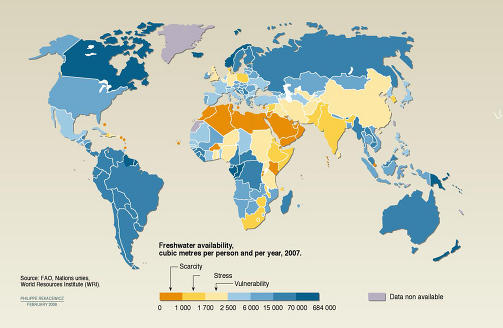
\includegraphics[width = 6cm]{picture/WaterScarcityMap.jpg}
  \end{wrapfigure}
  which make it a region where water is moderately overloaded. In our consideration, level 2, will provide more abundant behavior in a dynamical model(will it become water scarce or water sufficient in the future?). Thus we pick up China as our research object. To make our model more predictable and more reality connected. We will continue our investigation with the data from National Bureau of Statistics of the People's Republic China\cite{ChinaDataBase}.
  According to our models, the following variables are prominent: the Population, the GDP, the water consumption and the total water resource.
  We grab all the data and try to analyses them and they relation.

  \subsection{Prominent variables' tendency}

  \subsection{Prominent variables' relation}

  \subsection{fitness of past data using dynamic model}


\section{Prediction of water situation}
  In our model external variables are used for future prediction.


\section{Intervention plan designing}

\section{Prediction with Intervention plan}

\section{Conclusion}


\begin{thebibliography}{99}
  \bibitem{AbilityMeasure} {Falkenmark and Lindh 1976, quoted in UNEP/WMO.Climate Change 2001: Working Group II: Impacts,Adaptation and Vulnerability. UNEP. Retrieved 3 February 2009.}
  \bibitem {WaterScarcityMap} http://www.unep.org/dewa/vitalwater
  \bibitem{WaterCycle} trinityrivertexas.org, Living with the Trinity Lesson Plan 1: The Natural Water Cycle and the Urban Water Cycle
  \bibitem{ChinaDataBase} http://www.stats.gov.cn
\end{thebibliography}


%==========================================================

\begin{comment}
%===============================appendices===============================
    \begin{appendices}
    %\renewcommand{\thesection}{\Alph{chapter}.}

      \section{First appendix}

    some text...


Here are simulation programmes we used in our model as follow.\\


\textbf{\textcolor[rgb]{0.98,0.00,0.00}{Input matlab source:}}
\lstinputlisting[language=Matlab]{./code/matlab1.m}


      \section{Second appendix}

    some more text\textcolor[rgb]{0.98,0.00,0.00}{\textbf{Input C++ source:}}
\lstinputlisting[language=C++]{./code/sudoku.cpp}

    \end{appendices}

\end{comment}